\documentclass{beamer}
\usepackage[utf8]{inputenc}
\usepackage{graphicx}
\usepackage{color}
\newcommand{\hilight}[1]{\textbf{\textcolor{structure.fg!85}{#1}}}
\usepackage{hyperref}
\hypersetup{
    colorlinks=true,
    linkcolor=blue,
    filecolor=magenta,      
    urlcolor=cyan,
}

\setbeamertemplate{footline}[frame number]

\author[Sowmya Vajjala]{Sowmya Vajjala}

\title[SfSNLP]{NLP without Annotated Dataset}
\subtitle{Course Overview}
%: \\ on using insights from language acquisition, cognitive science and psychology research

\date{8 January 2021}

\institute{Seminar f\"ur Sprachwissenschaft, University of T\"ubingen, Germany}
%%%%%%%%%%%%%%%%%%%%%%%%%%%

\begin{document}

\begin{frame}\titlepage
\end{frame}

\begin{frame}
\frametitle{Today's plan}
\begin{itemize}
    \item Course overview
    \item NLP overview
\end{itemize}
\end{frame}


\begin{frame}
\frametitle{}
\bigskip
\Large Course Overview
\end{frame}

\section{Introduction}
\begin{frame}
\frametitle{About me}
\begin{itemize}
\item I work as a full time researcher at the National Research Council, Canada in Digital Technologies Research Center.
\item 2020: Wrote a book for O'Reilly (http://www.practicalnlp.ai/)
\item 2018-19: Senior Data Scientist in software engineering r\&d teams in Toronto
\item 2016-18: Assistant Professor (tenure track) at Iowa State University, USA
\item 2011-15: PhD at University of Tuebingen, Germany
\item Before that: software developer, Bachelors/Masters in Engineering
\end{itemize}
\end{frame}

\begin{frame}
\frametitle{About You}
\begin{itemize}
\item 22/46 filled the questionnaire so far (at 1600 CET).
\item Mostly MA, followed by BA ISCL?
\item Background: Mostly Linguistics, and many wrote they know some programming. 
\item Languages you speak: English, German, Italian, Spanish, Portuguese, Swedish, Arabic, Russian, Mandarin, Korean,Japanese, Thai, Bahasa Indonesia, Acehnese! \pause
\item Why are you enrolled in this course? What do you want to do later?
\begin{itemize}
\item A common answer: learn practical aspects of NLP and work in the industry
\item Do research on NLP for native languages (non English/German)
\end{itemize}
\end{itemize}
\end{frame}

\begin{frame}
\frametitle{Teaching experience}
\begin{itemize}
\item 2011-13: 2 Hauptseminar courses at Tuebingen (with Prof Meurers)
\item 2016-18:
\begin{itemize}
\item Applied Linguistics grad students: Python programming, Introduction to NLP
\item Grad Computer science students: Statistical NLP
\item Undergrad students from all disciplines : "Language and Computers", "Text as Data" (R), Technical Communication 
\end{itemize}
\item 2020: Guest course at Munich Graduate School of Economics, Germany (online)
\end{itemize}
\end{frame}

\begin{frame}
\frametitle{Course Background}
\begin{itemize}
\item NLP is a part of many day to day applications we use, such as search engines, virtual assistants on your smartphones and various functionalities in your email.
\pause \item When we think of NLP, we think of the various algorithms, neural network architectures, and so on. \pause
\item However, what drives all of them are large collections of annotated corpora. \pause
\item What do you do when you don't have access to such datasets, though? 
\end{itemize}
\end{frame}

\begin{frame}
\frametitle{Course Objectives}
\begin{itemize}
\item Provide an overview of NLP system development pipeline
\item Discuss some common approaches for collecting, cleaning and exploring text data
\item Introduce some methods to develop labeled data for NLP 
\end{itemize}
\end{frame}

\begin{frame}
\frametitle{Expected Learning Outcomes}
Students should be able to: 
\begin{itemize}
\item Understand the end to end NLP system development pipeline
\item Compile and explore labeled/annotated corpora for NLP
\item Build some basic text classification and information extraction systems
\end{itemize}
... upon successful completion of the course..
\end{frame}

\begin{frame}
\frametitle{Pre-requisities}
\begin{enumerate}
\item Intermediate proficiency in any programming language (Python preferred)
\item Comfortable installing libraries etc on their laptops
\item Knowledge of the usage of virtual environments (venv, anaconda) is useful
\end{enumerate}
\end{frame}

\begin{frame}
\frametitle{What the course can't do}
\begin{itemize}
\item Don't expect to become an NLP expert with one compact course. 
\item Contents may not always meet your own expectations, but there is a term paper and a group discussion, which gives you opportunities to explore your specific interests related to this topic.
\item The course won't teach you programming. 
\end{itemize}
\end{frame}

\begin{frame}
\frametitle{How we learn and grow}
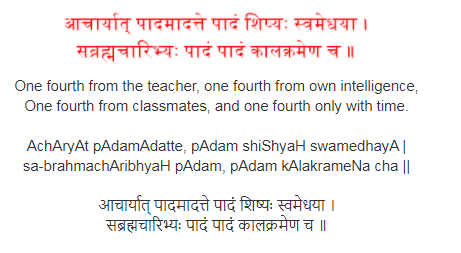
\includegraphics[width=\textwidth]{figures/acharyat.PNG}
\href{https://blog.practicalsanskrit.com/2009/12/how-we-learn-and-grow.html}{Source}\end{frame}

\begin{frame}
\frametitle{}
\begin{center}
\Large Course Logistics
\end{center}
\end{frame}

\begin{frame}
\frametitle{Meeting and Location}
\begin{itemize}
\item January 8 2021-January 29, 2021, M W F, 17:00 s.t. - 19:30 (Central European Time). 
\begin{enumerate}
    \item 8th Jan 2021 (Friday)
    \item 11th, 13th, 15th Jan 2021 (Mon, Wed, Fri)
    \item 18th, 20th, 22nd Jan 2021 (Mon, Wed, Fri)
    \item 25th, 27th, 29th Jan 2021 (Mon, Wed, Fri)
\end{enumerate}
\item Location: Zoom Meeting-ID: 990 5086 7382     \\                                   
Kenncode: 296817    
\item For a one to one meeting, email me to set up a time. I am keeping 1700-1800 free on most days in January for these one to one meetings. 
\end{itemize}
\end{frame}

\begin{frame}
\frametitle{Course Website}
\begin{itemize}
\item Moodle: \url{https://moodle.zdv.uni-tuebingen.de/course/view.php?id=1301}
\item Syllabus, Lecture slides and Assignments will be uploaded there.
\end{itemize}
\end{frame}

\begin{frame}
\frametitle{Course Format + Credits}
\begin{itemize}
\item Video lectures + Discussion (I may sometimes pick people randomly and ask a question!)
\item Assignments (2)
\item Team presentations: You are expected to form into groups of 2-4 people, pick a paper from the reading list on the website (or any other relevant paper) and present a brief discussion in a live session (10-15 minutes per group)
\item Assignments 
\item Term paper(optional)
\end{itemize}
Credits: 3 CP (+ 3 CP if you write a term paper)
\end{frame}

\begin{frame}
\frametitle{Textbooks}
\begin{enumerate}
\item "Speech and Language Processing" by Jurafsky and Martin (2/3 editions)
\item "Practical Natural Language Processing" by Sowmya Vajjala, Bodhisattwa Majumder, Anuj Gupta and Harshit Surana.
\item NLTK book
\item For Python: "Python for Everybody" Charles Severance 
\end{enumerate}
(Details on how to access these books are in the Syllabus document)
\end{frame}

\begin{frame}
\frametitle{Course Topics}
\begin{enumerate}
\item Introduction (1 session)
\item NLP Pipeline (1 session)
\item Corpus collection, extraction, exploration (1 session)
\item Automatically labeling data (3 sessions)
\end{enumerate}
remaining 4 sessions are for student presentations and review.
\end{frame}

\begin{frame}
\frametitle{Assignments/Grading (for 6 CP)}
\begin{enumerate}
\item 2 Assignments (30\% of the grade)
\item 1 presentation (30\% of the grade)
\item 1 term paper (30\% of the grade)
\item classroom participation (10\% of the grade)
\end{enumerate}
(For 3 CP: Split the term paper grade between two assignments)
\end{frame}

\begin{frame}
\frametitle{Assignments}
\begin{itemize}
\item Two assignments, already uploaded on Moodle
\item They are not difficult - the goal is not to trick you, but to make you think about the challenges of working with NLP problems in real world.
\item My preferred programming language is Python, I am okay with Java, R, C, C++, and anything else (note: I can't debug for you. What you submit should run error-free on my machine). 
\end{itemize}
\end{frame}

\begin{frame}
\frametitle{Presentation}
\begin{itemize}
\item Students can work in teams of 2-4 people and present one of the research papers related to course topics, from a given list of papers.
\item Papers are listed in the syllabus document. If you want to present a different paper, talk to me first. 
\item Pick your teams early (deadline: 13th Jan)
\end{itemize}
\end{frame}

\begin{frame}
\frametitle{Term Paper}
\begin{itemize}
\item Work on a short project involving NLP and write  a report describing your work (6-8 pages long in single column, latex formatted document)
\item Some ideas are listed in the syllabus document. If you want to work on something else, talk to me first. 
\item If you want to get into NLP research later, explore some of your ideas through this term paper!
\end{itemize}
\end{frame}

\begin{frame}
\frametitle{Classroom Participation}
\begin{itemize}
\item Attending live meetings
\item Participating in the forum
\item Communicating (Asking questions, informing me if something comes up and you can't attend etc)
\item Submitting stuff on time
\end{itemize}
\end{frame}

\begin{frame}
\frametitle{Important Deadlines}
\begin{enumerate}
    \item Decide on a team for group discussion (13th Jan 2021)
    \item Decide on a paper for group discussion (15th Jan 2021)
    \item Group Discussions (22nd-27th Jan 2021)
    \item Assignments 1 and 2 Submission (6th Feb 2021)
    \item Decide on term paper topic (29th Jan 2021)
    \item Term paper submission (13th Feb 2021)
\end{enumerate}
\end{frame}

\begin{frame}
\frametitle{}
\begin{itemize}
    \item Questions so far?
\end{itemize}
\end{frame}

\end{document}



